\section{Results}
An important property of any benchmarking method is the variance of the datasets from which these benchmarks are drawn. Small variance will magnify small discrepancies between students and as such does not provide a useful means of assessing students for university admission. Obviously the higher the degree of correlation between benchmarking methods and course grades the better.

An ideal benchmark has a high degree of correlation with a large variance. Obviously benchmarking methods should be applicable to as large a group of students as possible (for example, although additional mathematics may be a good means of assessing incoming student's abilities, it is useless since so few students take this subject in matric).

\subsection{Variance}
Only admissions data with values for all Gr12 grades (except math literacy and additional maths) and NBT results were considered resulting with a sample size of \mintinline{text}{n = 908} students over 3 years.

\subsection{Benchmark / Grade Correlation}
Correlation between the Grades and various combinations of the Benchmarks data shows that compared to Gr12 results, the NBT scores correlate better with CSC1015F performance. The highest correlation between benchmarking and CSC1015F course results occurs when the NBT scores are averaged, with either the NBT QL or NBT Mth (or both) scores double weighted; such a correlation is 0.50, which is considered a moderate correlation.

\subsection{LMS Usage}
Because the event data doesn't contain a foreign key to the grade entities, it is only possible assess the count of presence events for all sites in relation to the CSC1015F site. This isn't particularly useful, and perhaps is the main reason that no correlation is found. However this analysis is useful in demonstrating how such a correlation can be performed using CouchDB making such an analysis somewhat worthwhile.

Taking the NBT QL benchmark as an example (which has a comparatively high correlation with course grades compared to other benchmarks), the \( \delta \) class rank of benchmark score vs grade score is plotted against presence event count of each student in \ref{fig-delta-rank} for a visual feel of how the correlation analysis plots. The correlation between course grades (for CSC1015F) and LMS usage is relatively insignificant according to these results.

\begin{figure}[H]
    \centering
    % \begin{mdframed}
    % \centering
    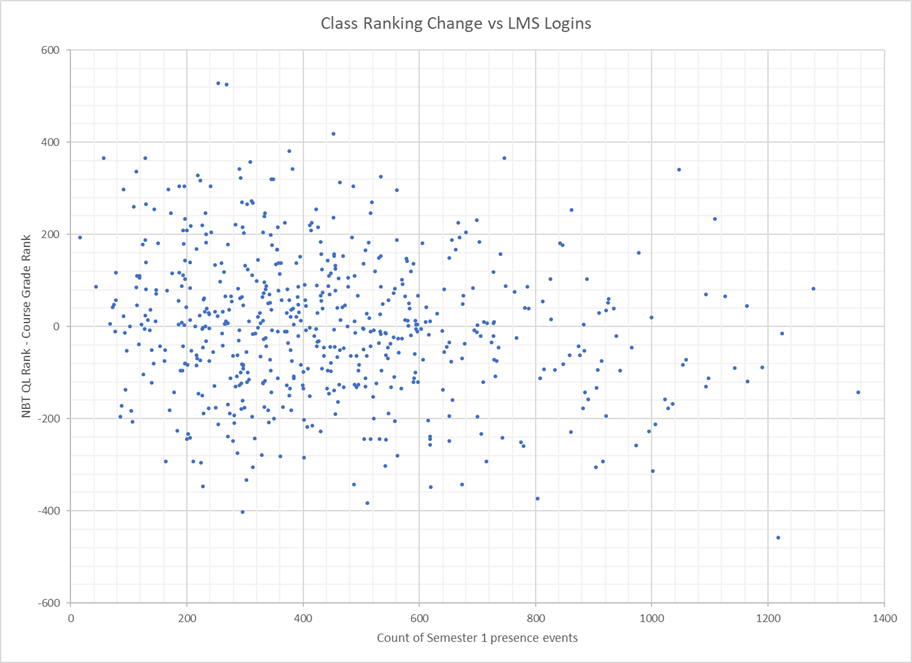
\includegraphics[scale=0.6]{./resources/figures/delta-class-rank.png}
    % \end{mdframed}
    \caption[\( \delta \) class rank vs LMS Logins]{\textbf{Figure \ref{fig-delta-rank}: \( \delta \) class rank vs LMS Logins.} An example of the correlation between \( \delta \) NBT QL ranking scores/course grades compared to LMS usage. As shown in Table \ref{tbl-correlation-variance}, the correlation coefficient between these two datasets is 0.17.}
    \label{fig-delta-rank}
\end{figure}